\documentclass[25pt, a0paper, landscape]{tikzposter}
\tikzposterlatexaffectionproofoff
\usepackage[utf8]{inputenc}
\usepackage{authblk}
\usepackage{setspace}

% for jpeg pictures
\usepackage[]{graphicx}
\makeatletter
\renewcommand\maketitle{\AB@maketitle} % revert \maketitle to its old definition
\renewcommand\AB@affilsepx{\quad\protect\Affilfont} % put affiliations into one line
\makeatother
\renewcommand\Affilfont{\Large} % set font for affiliations
\usepackage{amsmath, amsfonts, amssymb}
\usepackage{tikz}
\usepackage{pgfplots}
% align columns of tikzposter; needs two compilations
\usepackage[colalign]{column_aligned}

% tikzposter meta settings
\usetheme{Default}
\usetitlestyle{Default}
\useblockstyle{Default}

\usepackage[active,tightpage]{preview}
\usepackage{pgfplots}
\pgfplotsset{compat=newest}
\PreviewEnvironment{tikzpicture} 

%Bib einrichten
%\bibliographystyle{plain}
%\bibliography{bibli}



	
	
\definecolor{tb_color_1}{RGB}{245,124,0}
\definecolor{tb_color_2}{RGB}{0,167,247}
 

\definecolor{tb_color_1}{RGB}{245,124,0}
\definecolor{tb_color_2}{RGB}{0,167,247}

\pgfplotscreateplotcyclelist{tb}{
	semithick,tb_color_1\\%
	semithick,tb_color_2\\%
}
%%%%%%%%%%% redefine title matter to include one logo on each side of the title; adjust with \LogoSep
\makeatletter
\newcommand\insertlogoi[2][]{\def\@insertlogoi{\includegraphics[#1]{#2}}}
\newcommand\insertlogoii[2][]{\def\@insertlogoii{\includegraphics[#1]{#2}}}
\newlength\LogoSep
\setlength\LogoSep{-70pt}

\renewcommand\maketitle[1][]{  % #1 keys
	\normalsize
	\setkeys{title}{#1}
	% Title dummy to get title height
	\node[inner sep=\TP@titleinnersep, line width=\TP@titlelinewidth, anchor=north, minimum width=\TP@visibletextwidth-2\TP@titleinnersep]
	(TP@title) at ($(0, 0.5\textheight-\TP@titletotopverticalspace)$) {\parbox{\TP@titlewidth-2\TP@titleinnersep}{\TP@maketitle}};
	\draw let \p1 = ($(TP@title.north)-(TP@title.south)$) in node {
		\setlength{\TP@titleheight}{\y1}
		\setlength{\titleheight}{\y1}
		\global\TP@titleheight=\TP@titleheight
		\global\titleheight=\titleheight
	};
	
	% Compute title position
	\setlength{\titleposleft}{-0.5\titlewidth}
	\setlength{\titleposright}{\titleposleft+\titlewidth}
	\setlength{\titlepostop}{0.5\textheight-\TP@titletotopverticalspace}
	\setlength{\titleposbottom}{\titlepostop-\titleheight}
	
	% Title style (background)
	\TP@titlestyle
	
	% Title node
	\node[inner sep=\TP@titleinnersep, line width=\TP@titlelinewidth, anchor=north, minimum width=\TP@visibletextwidth-2\TP@titleinnersep]
	at (0,0.5\textheight-\TP@titletotopverticalspace)
	(title)
	{\parbox{\TP@titlewidth-2\TP@titleinnersep}{\TP@maketitle}};
	
	\node[inner sep=0pt,anchor=west] 
	at ([xshift=-\LogoSep]title.west)
	{\@insertlogoi};
	
	\node[inner sep=0pt,anchor=east] 
	at ([xshift=\LogoSep]title.east)
	{\@insertlogoii};
	
	% Settings for blocks
	\normalsize
	\setlength{\TP@blocktop}{\titleposbottom-\TP@titletoblockverticalspace}
}



\makeatother
%%%%%%%%%%%%%%%%%%%%%%%%%%%%%%%%%%%%%


% color handling
\definecolor{TumBlue}{cmyk}{1,0.43,0,0}
\colorlet{blocktitlebgcolor}{TumBlue}
\colorlet{backgroundcolor}{white}

% title matter
\title{Tetris - Reinforcement Learning$^2$}

\author[ ]{Sebastian Fellner, Simon Speth, Benedikt Wiberg, Paul Kehnel}
%\author[ ]{Simon Speth}
%\author[1]{Benedikt Wiberg}
%\author[1]{Paul Kehnel}
%
%\affil[1]{Technical University of Munich}

\insertlogoi[width=15cm]{tum_logo}
\insertlogoii[width=15cm]{tum_logo}

% doesnt work for me with compat=1.14
% \pgfplotsset{compat=1.14}
% main document
\begin{document}
	
	\stepcounter{footnote}
	\renewcommand\thempfootnote{\arabic{footnote}}
	
	\maketitle
	
	\begin{columns}
		\column{0.25}
		\block{Motivation}{
			\begin{minipage}{\linewidth}
			\textbf{Why reinforcement learning with Tetris?}

			Deepmind has shown in several papers that it is possible to use the same Deep {Q-Network} (DQN) to solve different atari 2600 games on a superhuman level\footnote{Mnih, Volodymyr, et al. "Playing atari with deep reinforcement learning." arXiv preprint arXiv:1312.5602 (2013).}.
			\stepcounter{footnote}
			\renewcommand\thempfootnote{\arabic{footnote}}


			It would be interesting to see if it is possible to transfer these techniques to a game that requires deeper understanding of the game mechanics. Because of the great variance of possible stones and the resulting task of planning Tetris is an NP-Hard problem\footnote{Erik D. Demaine and Susan Hohenberger and David Liben{-}Nowell, Tetris is Hard, Even to Approximate,CoRR 2002.}.

			\stepcounter{footnote}
			\renewcommand\thempfootnote{\arabic{footnote}}

			We set our task to use Reinforcement Learning (RL) with Convolutional Neural Networks
			(CNN) to learn optimal control policies for Tetris.

		\end{minipage}
		}

		\block{Related Work}{
			\begin{minipage}{\linewidth}
			\begin{itemize}
%				\item \textbf{Learning Tetris using the noisy cross-entropy method:}\footnote{Szita, I. and L{\"o}rincz, A., 2006. Learning Tetris using the noisy cross-entropy method. Neural computation, 18(12), pp.2936-2941.} This is one of the older approaches. They apply noise for preventing early convergence of the cross-entropy method, by that optimising and outperforming previous RL algorithms.
%				% increment footnote
%				\stepcounter{footnote}
%				\renewcommand\thempfootnote{\arabic{footnote}}
				
				\item \textbf{Playing Atari with Deep Reinforcement Learning:}\footnote{Mnih, Volodymyr, et al. "Playing atari with deep reinforcement learning." arXiv preprint arXiv:1312.5602 (2013).} This paper by Deepmind is one of the most impressive works on Reinforcement Learning and can be seen as fundamental work for further improvements.
				
				% increment footnote
				\stepcounter{footnote}
				\renewcommand\thempfootnote{\arabic{footnote}}
				
				\item \textbf{Rainbow: Combining Improvements in Deep Reinforcement Learning:}\footnote{Hessel, Matteo, et al. "Rainbow: Combining Improvements in Deep Reinforcement Learning." arXiv preprint arXiv:1710.02298 (2017).} This is the current state of the art, by combining different enhancements for DQN. This is crucial for selecting well fitting enhancements for our problem.

				% increment footnote
				\stepcounter{footnote}
				\renewcommand\thempfootnote{\arabic{footnote}}
			\end{itemize}
		\end{minipage}
	}
	
	\block{Mathematical Background}{		
		\textbf{Bellman equation:} Used to derive a recursive decomposition of the optimal $q$-value function.
		$Q^*$ returns for the state $s$ and the action $a$ the expected discounted future reward.
		
		 $Q^*(s,a) = \mathbb{E}_{s' \sim \mathcal{E}}[r + \gamma \max_{a'}{Q^*(s',a')|s,a}]$
		 
		 

		\textbf{Loss Function:} We use the same loss function as presented in the Double DQN Paper from Hado van Hasselt.
		
	\begin{align*}
	\text{	\textbf{Reward Function}}\ \ r(x)  =
	\begin{cases}
	-1 & \text{if dead,}\\
	n/(h+1) & \text{if line cleared,}\\
	0.01 & \text{else}  
	\end{cases}
	\end{align*}

	$n$: number of lines cleared, $h$: maximum board height.
	}
\column{0.45}
\block{Approach}{
	\begin{minipage}[t]{\linewidth}
		\begin{minipage}[t]{0.6\linewidth}
			\textbf{The Beginning}:
			Our first approach was using the proposed architecture from the Deepmind Atari Paper on a high resolution standard tetris implementation. 
			Due to the high resolution input and the high variance betweeen stones the learning was slow and didn't converge.
			%\begin{itemize} 
			%	\item Setup of synchronous Tetris-Gym-Environment (with all standard tetrominos), that fulfills the required markov property (see Figure 1)
			%	\item Action-space: move\_stone\_left, move\_stone\_right, rotate\_stone, instant\_down, nothing (and allways one step down)
			%	\item State-space: High resolution RGB-image ($110 \text{px} \times 220 \text{px}$) of Tetris-game (each stone has a differen colour)
			%	\item Architecture and Algorithm: different implementations of DQN with and without enhancements
			%\end{itemize}
			\\
			\\
			\textbf{Initial Improvements}:
			By downscaling the input to 1 block per pixel and removing unneeded color information, we could achieve much higher iteration rates. Further simplification of tetris to a 5x11 board with only two different stones (
\includegraphics{images/tetrinos2.pdf} and 
\includegraphics{images/tetrinos3.pdf}) provided us with an environment with very good convergence rates to test different architectures. While this version of tetris is easier to play, we achieved comparable performance on the normal 10x22 tetris board with the same architectures. 
		\end{minipage}
		\hspace{1em plus 1fill}
		%\quad
		\begin{minipage}[t]{0.35\linewidth}
			\vspace{-2ex}
			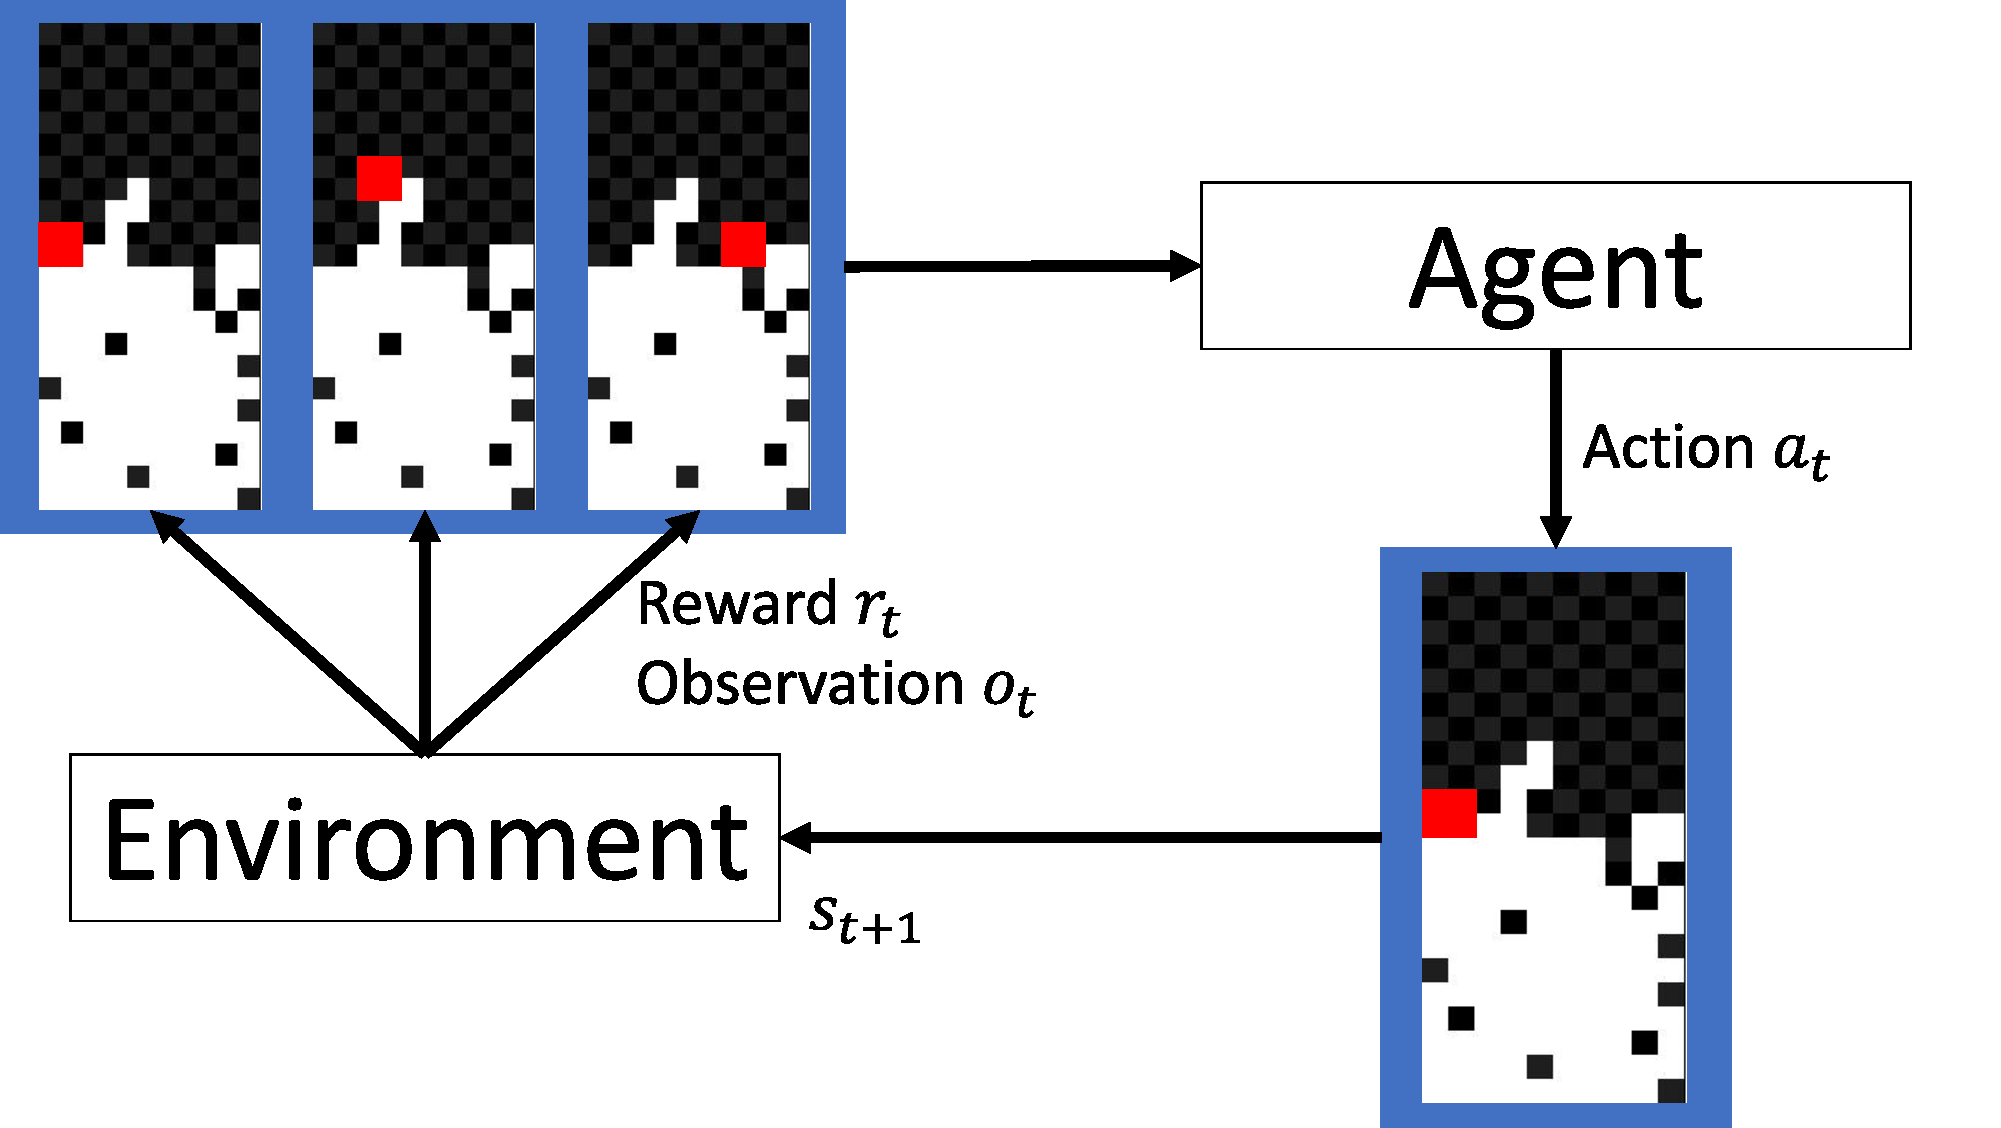
\includegraphics[width=\linewidth]{images/agent_env_loop}
			\begin{small}
				{\textbf{Figure 1: \label{fig:environment}}  Setup of our Tetris-environment: The agent selects action $a_t$ at time $t$, the environment computes reward $r_t$, observation $o_t$ and new state $s_{e,t+1}$ with respect to $a_t$ and $s_{e,t}$. In our case: $s_{a,t} = \emptyset$ and $s_{e,t} = o_t$ (the agent has no internal state and the agent observes the hole state space of the environment).}
			\end{small}
		\end{minipage}
		
	\end{minipage}
	
	%\begin{itemize}
	%	\item Simplified Tetris: Only one Stone (
\includegraphics{images/tetrinos1.pdf} 1x1 tetrino) with reduced field size and less actions (no instant drop down). As expected we could solve this pretty fast.
	%	\item Medium complex setup: In addition to the 
\includegraphics{images/tetrinos1.pdf} two other stones (
\includegraphics{images/tetrinos2.pdf} and 
\includegraphics{images/tetrinos3.pdf}) were added. This setup could not be solved by allowing the agent choose consecutive actions and move the stone. Even a fitnessfunction with different metrics to estimate the state value didn't help.
	%\end{itemize}
	\textbf{Problem of planning}:
			Tetris is mainly a problem of planning stone placements. Because each placement can consist of up to 22 actions, this leads to very sparse rewards. To combat this issue, we used a modified tetris environment where each action is equal to one possible placement position. Different game states have different amounts of total possible actions, so we needed a custom architecture. Instead of learning normal Q-values  $Q^*(s,a)$  for each possible action $a$ from the state $s_t$, we instead directly learn the Q-value of the state $[s_{t+1}|a_{t}]$ under the assumption that we picked action $a_t$. While we need to evaluate each possible next state individually, the gains in faster convergence rates outweight the slower inference.
	%\textbf{Breakthrough}:
	%\begin{itemize}
	%	\item InstaTetris-Environment: the agent now chooses the final position and rotation of the current stone instead of navigating it. Also, the input was reduced to one channel (only three different values: the current stone, background and positioned stones)	
	%	\item Multiple enhancements: Double-DQN, limit the game length to ensure the uncorrelation of the data in the experience buffer, simple network architecture
	%\end{itemize}
}
		\block{Network Architecture}{
		\centering	
    	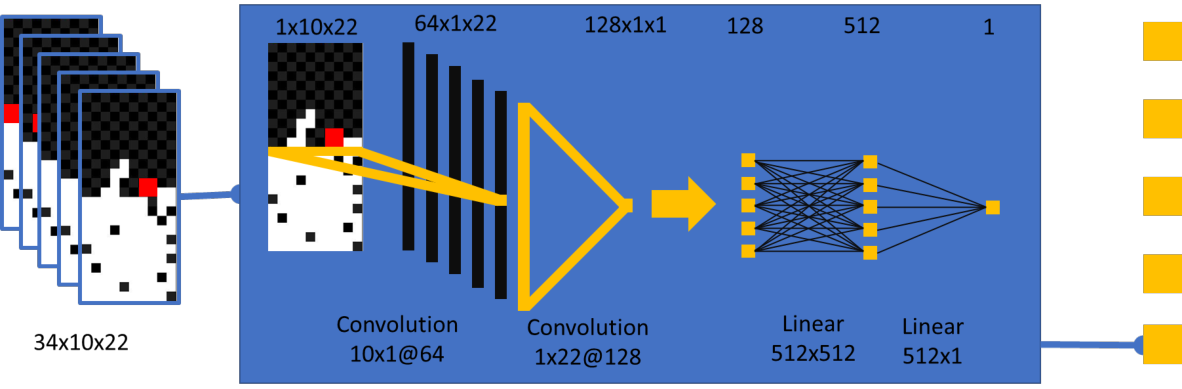
\includegraphics[width=\linewidth]{images/network}
		\begin{minipage}[t]{\linewidth}
			We employ a custom architecture using 1 dimensional convolutions to quickly reduce spatial size. After two additional
			linear layers we are left with the q-value of the proposed action. All layers except the last one use ReLU as the
			activation function. To address all possible tetromino placements, a batch of data consists of 34 possible placements\footnote{This represents the possible upper limit for different actions with a single stone on 10 wide board.}
			where the score is computed in parallel. In the end, the placement with the highest score is choosen and executed
			with regard to an $\epsilon$-greedy policy.
			\end{minipage}
			 %increment footnote
					\stepcounter{footnote}
					\renewcommand\thempfootnote{\arabic{footnote}}
		}            

		\column{0.3}
		\block{Results}{
			In the left graph one can see a linearly increasing mean summed reward for the first 3 mio. training steps. We expect the curve to increase even further with a longer tarining phase. Unfortunately time was limited.
			
			The right hand graph shows the evaluation of a randome agent (red) and our trained model (blue) with a maximum reward of 110 in a single game. 
				 
				\begin{tikzpicture}
				\begin{axis}[cycle list name=tb, 
				title=Training,
				grid=both,
				width=10cm,
				height=10cm,
				grid style={solid,gray!30!white},
				axis lines=middle,
				xlabel={Steps},
				%ymax = 10,
				align =center,
				ylabel = {Mean Summed\\Reward ($\phi_{100}$)},
				tick label style = {font=\tiny},
				x label style={at={(axis description cs:0.5,-0.2)},anchor=north},
				y label style={at={(axis description cs:-0.3,.5)},rotate=90,anchor=south},]
				\addplot [TumBlue] table [x=Step, y=Value, col sep=comma] {images/graphs/training_v2.csv};
				\end{axis}
				\end{tikzpicture}
				\begin{tikzpicture}
				\begin{axis}[cycle list name=tb, 
				title=Evaluation,
				width=10cm,
				height=10cm,
				grid=both,
				grid style={solid,gray!30!white},
				axis lines=middle,
				xlabel={Games},
				tick label style = {font=\tiny},
				ymax = 150,
				%ymin = -1,
				align =center,
				ylabel={Summed\\Reward\\},
				x label style={at={(axis description cs:0.5,-0.2)},anchor=north},
				y label style={at={(axis description cs:-0.0,.5)},rotate=90,anchor=south},]
				\addplot [red] table [x=Step, y=Value, col sep=comma] {images/graphs/random_baseline.csv};
				\addplot [TumBlue] table [x=Step, y=Value, col sep=comma] {images/graphs/evaluationwithtrainingrewardfunction2.csv};
				\addlegendentry{baseline}
				\addlegendentry{trained agent}
				\end{axis}
				\end{tikzpicture}
		}
		\block{Conclusion}{
			\begin{enumerate}
				\item To benchmark our agent performance we compared it to a random playing agent, another implementation of two students from Stanford and a (near) Perfect Bot.
				Since the bot can play forever we compare the average number of lines deleted after 1000 placed tetrominos.
				\begin{tabular}{|c|c|c|c|c|} \hline
					\textbf{Name:}& Our Agent & Random & Stanford & Perfect Bot \\ \hline
					Lines per 1000 tetrominos & 92 & $ 1 $ & 21 & 200 \\ \hline
				\end{tabular}
%				\item Since the normal version even in earlier staged showed the same behaviour as the simple version, we assumed that it will also converge, but logically needed way more time.
				\item The network architecture from DQN was not really transferable. On the one hand we did not need to apply downconvolution to the input, since it was already small enough ($22 \text{px} \times 10 \text{px}$) and on the other hand it seems like more computing time would not solve the problem completely. DeepMind trained for 50 mio steps (ca. 30 days).
				\item Further work: As a next interesting step "blind Tetris" could be to approached. Therefore we would recommend using a Recurrent Neural Network (RNN). Also transfer learning would be an interesting topic, that could possibly lead to much faster learning success. The idea would be that you start with one tetromino and once the agent plays optimal you would add another tetromino and so on.
			\end{enumerate}

			\begin{minipage}[t]{\linewidth}
				\textbf{Other work and gimmicks:}
					\begin{itemize}
					\item Implementation of a simple Human Tetris environment for a good comparison and in preparation for supervised learning.
					
				\end{itemize}
				\begin{minipage}[t]{0.5\linewidth}

					\begin{itemize}
						\item Approaches of supervised learning, where we prefilled the experience buffer with recorded games played in the simple Human environment.
						\item Using Tensorboard for statistcs and evaluation.
						\item Twitch Live Stream to follow the learning progress.
					\end{itemize}
				\end{minipage}
				%\quad
				\begin{minipage}[t]{0.5\linewidth}
					\vspace{-2ex}
					\centering
					
\includegraphics[width=0.5\linewidth]{images/QRCode.pdf}
					\begin{small}
					www.twitch.tv/koztantwo
					\end{small}
				\end{minipage}
			\end{minipage}
		}

	\end{columns}
\end{document}
